\documentclass[aspectratio=1610,svgnames]{beamer}

\usepackage{lmodern}
\usepackage[T1]{fontenc}
\usepackage[ngerman]{babel}
\usepackage{selinput}
\SelectInputMappings{%
   adieresis={ä},
   germandbls={ß}
   }

\usetheme{PaloAlto}  %% Themenwahl

\setbeamercovered{transparent}
%\setbeamertemplate{footline}[frame number]
\usecolortheme{spruce}		% grün
\usecolortheme[named=MSUgreen]{structure}
\newcommand{\hshblogo}{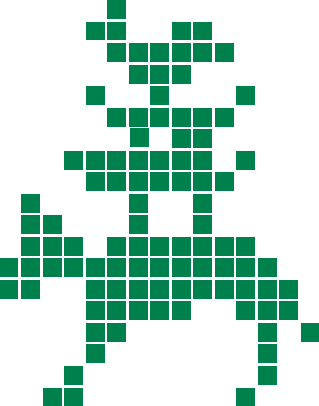
\includegraphics[width=1.3cm]{space-logo}}
\newcommand{\divider}[1]{\begin{frame} %
\begin{alertblock}{} %
\centering\usebeamerfont{section title}#1 %
\end{alertblock} %
\end{frame}}
 
\newcommand{\code}[1]{\texttt{#1}}

\title{3D Objekte mit OpenSCAD}
\author{Thomas Helmke}
\date{09.02.2016}
\logo{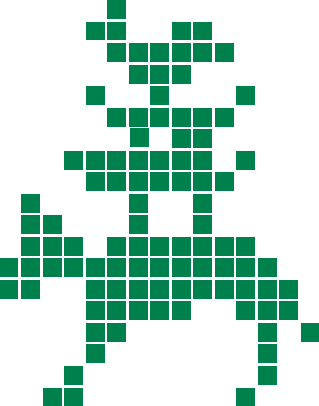
\includegraphics[width=1.1cm]{space-logo}}
 
\begin{document}
\maketitle
\frame{\tableofcontents}

\section{Einleitung}
\divider{\insertsection}
\begin{frame}%[<+->] %%Eine Folie
	\frametitle{Worum geht es?} %%Folientitel
	\begin{itemize}
		\item 3D Objekte entwerfen
        \item 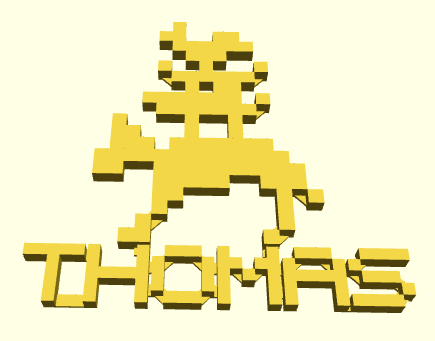
\includegraphics[width=0.3\textwidth]{nametagthomas}
		\item zum Beispiel für 3D Druck
	\end{itemize}
\end{frame}
\begin{frame}[<+->] %%Eine Folie
	\frametitle{openSCAD} %%Folientitel
	\begin{itemize}
		\item eine 3D CAD Software
        \item nicht interaktiv, sondern skriptbasiert
		\item freie Software, für alle Platformen erhältlich\footnote{\url{www.openscad.org}}
		\item fast vollständige JavaScript Version läuft direkt im Browser\footnote{\url{www.openscad.net}}
	\end{itemize}
\end{frame}

\section{Grundlagen}
\divider{\insertsection}
\subsection{Basiskörper}
\divider{\insertsubsection}
\begin{frame}[<+->]
    \frametitle{Basiskörper}
    \begin{itemize}
        \item Würfel -- \code{cube([xLänge, yLänge, zLänge]);}
        \item Zylinder -- \code{cylinder(h = Höhe, r1 = RadiusUnten, r2 = RadiusOben);}
        \item Kugel -- \code{sphere(r = Radius);}
    \end{itemize}
\end{frame} 
\begin{frame}[<+->]
    \frametitle{optionale Parameter}
    \begin{itemize}
        \item \code{center} -- zentriert den Körper im Koordinatenursprung
        \item \code{\$fn} -- Anzahl der Flächen für runde Körper
        \item \code{d} -- Durchmesser statt Radius
    \end{itemize}
\end{frame} 
\subsection{Basisoperationen}
\divider{\insertsubsection}
\begin{frame}[<+->]
    \frametitle{Basisoperationen}
    \begin{itemize}
        \item .
        \item .
        \item .
        \item .
    \end{itemize}
\end{frame} 

\section{Fortgeschrittene Techniken}
\divider{\insertsection}
\begin{frame}[<+->]
    \frametitle{Arduino Version}
    \begin{itemize}
        \item .
        \item .
        \item .
        \item .
    \end{itemize}
\end{frame}

\section{Scripting}
\divider{\insertsection}
\begin{frame}[<+->]
    \frametitle{Arduino Version}
    \begin{itemize}
        \item .
        \item .
        \item .
        \item .
    \end{itemize}
\end{frame}

\section{Weitere Infos}
\divider{\insertsection}
\begin{frame}
    \frametitle{Weitere Infos}
    \begin{itemize}
        \item \url{https://github.com/Syralist/hshb-pres-ledpixels}
        \item \url{https://wiki.hackerspace-bremen.de/projekte/videogame/start}
        \item \url{https://github.com/HackerspaceBremen}
        \item \url{https://gist.github.com/jh0ker/8a63a66d368d7b48c89d}
    \end{itemize}
\end{frame}
\end{document}
